\cotefile{134-2}
\scanpage{153}\mspage{8}%
le \inserted{\unsure{complexe|complexes} de} faisceaux $f^!(\Lambda_e)$ (où $f:X\unsure{\text{---}|\longrightarrow}\operatorname{Spec} k=e$) joue le rôle du \uline{complexe \unsure{des|de} chaines singulières sur} $X$ \uline{à coeff. dans} $\Lambda$, et $Rf_!(f^!{\unsure{\Lambda|\mathbb{\Lambda}}}_e)$ joue le rôle d'une \uline{homologie} $H_*(X/e)$, vis à vis bien sûr de coefficients sur $e$ qui soient des complexes de $\Lambda$-modules. Tu justifieras aisément cette assertion à l'aide des ``th. de dualité globale'', par un ou deux tours de passe-passe que je t'épargne ici.

\uline{Remarques} 1) Il n'y a pas à tronquer, ça marche en toutes dimensions

2) C'est (au moins du p\textsuperscript{t} de vue philosophie) lié au fait qu'on dispose pour les \unsure{coefficient|coefficients} envisagés \inserted{(\unsure{sous|sans}) condition de ``constructibilité\unsure{'')|)}} d'un th. de ``bidualité''\unsure{\deleted{)}|\textsuperscript{(*)}}, du moins sous réserve de résolution des singularités (mais Deligne m'a dit je crois qu'il sait le prouver sans ça) à valeurs dans un ``complexe dualisant'' $K_e$ \inserted{(sur $e$)} $\unsure{\text{--}|;|\text{--};|\underset{\text{;}}{\longleftarrow}}$ $K_X$ (sur $X$). Si p.ex. $\Lambda$ est ``autodual'' \inserted{(ou Gorenstein)} p.ex. $\Lambda=\mathbb{Z}/n\mathbb{Z}$, on peut prendre $K_e=\Lambda$, donc \inserted{le complexe dualisant} $K_X=f^!(K_e)$ n'est autre que le ``complexe \unsure{des|de} chaines singulières \unsure{à} \unsure{coeff.} \unsure{dans} $\unsure{\Lambda}$'' \illegible{1}
% archive sheet number: 153

\scanpage{154}\mspage{9}
3) On peut faire les ${=}\mathrm{s}$ choses pour des coeff tels que $\mathbb{Z}_{\ell}$ (Jouanolou, thèse -- non publiée je crains !)

\inserted{4) Ça marche pour $f:X\unsure{\dashv|\longrightarrow}S$ \unsure{prés.|pres.} finie séparé, si $f$ a des propriétés de ``locale trivialité cohomologique'' (propr. locales \uline{en haut}) p.ex. $f$ \uline{lisse} ; on trouve $\underline{H}_{*X/S}=Rf_{!}\,f^{!}(\Lambda_S)$.}

B) Artin et Mazur ont étudié, dans un esprit voisin du tien, \uline{l'autodualité} de la jacobienne d'une courbe relative $X/S$. Il faut les consulter pour les résultats précis, peut-être cela marche dès que $X/S$ est propre et plat de dim relative $1$ -- en tous cas c'est OK sur un anneau de valuation discrète à fibre \uline{générique} lisse. La fibre spéciale peut être très sauvage. (J'ai utilisé \deleted{\unsure{pour|leur}}leur résultat dans SGA \deleted{\unsure{3}}7 pour prouver, dans le cas des jacobiennes, une conjecture de dualité sur les groupes de composantes connexes associés \unsure{aux} \deleted{\unsure{de|des} \unsure{V.A.|VA.}} modèles de Néron de V.A. duales l'une de l'autre....)

\figure{\begin{tikzpicture}
\draw (0,0)--(1.80em,-0.025em);
\draw (.63em,-.29em)--(1.63em,-.29em);
\end{tikzpicture}}

\deleted{\unsure{C)}} Vers la fin des années 50\inserted{(ou début des 60 ?)}, alors que les grands fourbis cohomologiques ($f_{!},f^{!}$, coh. étale etc) sortaient à peine des limbes, le cours de Serre sur la théorie de \unsure{Rosenlicht} et \unsure{Lang} des \unsure{Jacobiennes|jacobiennes|Jacobienne}
% archive sheet number: 154

\scanpage{155}\mspage{10\makebox[0pt][r]{\tikz[baseline=0pt,overlay]{\draw (0.16em,0.70em) .. controls (0.16em,-0.37em) and (-1.16em,-0.39em) .. (-1.16em,0.44em);}}}
\unsure{généralisées|généralisés} \deleted{et plu\unsure{s}}\inserted{et le corps de classe ``\unsure{géométrique|géomrique|géomérique}''} (voir le livre de Serre), et plus tard sa théorie ``géométrique'' du corps de classe \uline{local} à coups de groupes \unsure{proalgébriques|pro.algébriques} (voir son article sur le sujet), m'avait fait réfléchir à des formulations cohomologiques de ces résultats\inserted{ et d'autres}, qui devaient être notamment de nature \inserted{``géom'' telle} que les résultats ``arithmétiques'' sur un corps de base (ou résiduel) $k$ \inserted{général (fini, p.ex)} se ramènent immédiatement par \unsure{descente|descent} au cas ``géométrique'' du corps de base $\bar{k}$. J'ai eu un échange de lettres avec Serre -- je ne sais si j'en retrouverai des copies, mais je me rappelle qu'il s'agissait de projets de théories assez ambitieux, \inserted{à coups de résidus généralisés, Jacobiennes gén. locales etc\unsure{,|;}} dans au moins trois directions différentes. Mais je ne suis jamais parvenu, malgré de nombreux essais, à accrocher une bonne volonté à un de ces programmes. Voici quelques mots sur eux :

C) Situation $X$ de type fini sur \uline{corps} $k$,

\noindent\begin{tabular}{@{}|p{0.94\linewidth}@{}}
Construction d'un complexe de jacobiennes généralisées $J_{*X/k}$ (de long. égale à $\dim X$)
\end{tabular}
% archive sheet number: 155

\scanpage{156}\mspage{11}
C'était un complexe de pro-groupes algébriques sur $k$, affines à l'exception de $J_0$ si je me rappelle bien, (\deleted{\unsure{qui}}$J_0$ avait comme partie abélienne la partie abélienne de $\underline{\mathrm{Alb}}_{X/k}$
\margin{\begin{tabular}{@{}|p{\dimexpr\marginparwidth-0.8em\relax}@{}}
\illegible{} de $X$, i.e on avait un \deleted{\unsure{f}}hom $X\longrightarrow\underline{H}_0$ universel pour les hom de $X$ dans des groupes loc. proalgébriques. Pour $X$ connexe, $\underline{H}_0$ est une ext. de $\mathbb{Z}$ par un groupe proalg. connexe.
\end{tabular}}
\tikz[baseline=0pt]{\draw (0,.95ex)--(-.25em,.45ex)--(-.06em,.55ex)--(-.22em,.10ex)--(-.07em,.19ex)--(-.15em,-.14ex);}la jacobienne généralisée ordinaire). Sa construction, inspirée du complexe résiduel, passait par des jacobiennes généralisées (en un sens \inserted{cohomologique} convenable) des localisés $\operatorname{Spec}\underline{O}_{X,x}$ de $X$ en ses différents points. Il est possible qu'en un premier temps, je me limitais au cas $X$ lisse. Le rôle cohomologique de ce complexe était celui d'un complexe d'\uline{homologie}
\[
\mathrm{H}^{i}(X,G_X)\simeq\mathbb{E}\mathrm{xt}^{i}(J_{*X/k},G)\tag*{\makebox[0pt][r]{\makebox[\linewidth][l]{\unsure{\ensuremath{\alpha})|a)|(*)}}}}
\]
mais pour quels coefficients ? Je pense que je devais \deleted{\unsure{me limiter,|me limiter} plus ou moins à des} \inserted{prendre des groupes alg. comm. $G$ quelconques mais travailler en top. de Zariski (malédiction !)\unsure{, --|,, \ensuremath{\top}|. --}} \deleted{$G$ connexes (brr !), ou \unsure{plutôt|plu tôt}} \inserted{même} dans le cas $G$ discret, je prenais néanmoins des $\mathrm{H}^{i}$ zariskiens -- cela donne des groupes de cohomologie un peu bêta, évidemment. Je réalisais qu'il faudrait travailler en coh etale ultérieurement, et que la construction\inserted{\unsure{$\times$|$x$}} des $J_{\deleted{\unsure{*}}iX/k}$ en serait évidemment modifiée. Quant à la \unsure{sig-}%
% archive sheet number: 156

\scanpage{157}\mspage{12}%
nification des $\mathbb{E}\mathrm{xt}^{i}$ (hyperext), à un moment où Serre avait développé le formalisme des groupes proalgébriques, on n'avait pas trop peur de le prendre là-dedans -- au sens d'une catégorie dérivée qui à ce moment là n'avait encore jamais été définie et étudiée en forme.... (On a fait quand même un peu de chemin depuis !) J'ai bien l'impression, à la suite de ces antiques cogitations, pour heuristiques qu'elles furent, qu'on doit pouvoir développer à l'heure actuelle une telle théorie des $J_{*X/k}$, en coh fppf disons, donnant une formule $(*)$ sans limitation sur le dim $i$ de la cohomologie. (NB mais $J_*$ ne s'arrête évidemment plus en $\dim X=n$, mais en dim $2n$. Il est possible néanmoins que les composants $J_i$ soient de dim $0$ pour $i>n$).

Je crois bien que la construction de $J_*$ ne commute pas au chgt de base, mais que dans la cat. dérivée seulement elle y commute.

D) Soit $\deleted{f}X:/k$ schéma lisse \inserted{\deleted{\unsure{si|sic}}} (pour simplifier) sur corps $k$, séparé de \unsure{V.f.|T.f.|t.f.}, \inserted{de dim. relative $d$,} et $n$ entier $>0$. Si $n$ est premier à la caract. et si $F$ est un
% archive sheet number: 157

\scanpage{158}\mspage{13}
faisceau de coeff. sur $X$ annulé par $n$, la dualité globale nous dit que $Rf_{\deleted{\unsure{*}}!}(F)$ et $Rf_*(R\underline{\mathrm{Hom}}\,(F,\mu_n^{\otimes d}))$ sont duals l'un de l'autre à valeurs dans $(\mathbb{Z}/n\mathbb{Z})_k$, p.ex. $Rf_!(\mathbb{Z}/n\mathbb{Z})$ et $Rf_*(\mu_n^{\otimes d})$, ou $Rf_!(\mu_n^{\otimes d})$ et $Rf_*(\mathbb{Z}/n\mathbb{Z})$, sont duals l'un de l'autre -- du moins modulo un shift d'amplitude $2d$ sur les dimensions. (Comme $\mathbb{Z}/n\mathbb{Z}$ est injectif sur lui-même, cela donne d'ailleurs des dualités parfaites
\[
R^{i}f_{\deleted{*}!}(F)\times R^{2d-i}f_*(\mathbb{R}\underline{\mathrm{Hom}}\,(F,\mu_n^{\otimes d}))\longrightarrow\mathbb{Z}/n\mathbb{Z}\big{)}.
\]

Si maintenant $n$ n'est plus supposé premier à la caractéristique, \inserted{p.ex \inserted{est} une puissance de $p=\mathrm{car}\,k>0$,} il semble que tout \unsure{s'écroule|s'ecroule}, à commencer qu'on ne sait plus \inserted{(pour $d>1$)} par quoi remplacer $\mu_n^{\otimes d}$... Le miracle assez extraordinaire, c'est que pour $d=1$ i.e. $X$ une courbe lisse, tout continue à marcher parfaitement, pourvu qu'on l'énonce avec soin ! Les premières vérifications se font p.ex. avec $F=\mathbb{Z}/p\mathbb{Z}$, $\mu_p$, $\alpha_p$, $X$ complète -- on trouve que c'est OK grâce essentiellement à l'autodualité de la jacobienne. On peut sophistiquer les exemples, en prenant des coefficients $F$ \uline{tordus}, et $X$ non complète -- on se convainc que ça marche toujours.! Simplement il faut faire attention qu'ici les ${\unsure{R|\mathbb{R}}}^if_*(F)$, $R^if_!(F')$ ont une structure ``continue'' (ce sont essentiellement des \unsure{groupes} \unsure{ind-pro-algébriques)}
% archive sheet number: 158

\scanpage{159}\mspage{14}
Cela correspond au phénomène bien connu dans la théorie du corps de \unsure{classe|classes} que la structure du $\pi_{1\,\mathrm{ab}}$ de $X$, quand $X$ est non complète, est \uline{\unsure{continue|infinie}} -- donc il en est de $\bar{\mathrm m}$ du $\mathrm{H}^{1}(X,\mathbb{Z}/p^{n}\mathbb{Z})$ disons.

À ce propos, je te signale que Serre avait proposé (sans jamais l'écrire, je crois) une théorie de dualité des groupes algébriques commutatifs unipotents\inserted{ \unsure{connexes|connexe}}, \deleted{\unsure{duals|doubles|dualité}} pris \uline{mod isogénie radicielle}, dualité à valeurs dans $\mathbb{Q}/\mathbb{Z}$ (ou $\mathbb{Q}_p/\mathbb{Z}_p$). Il trouve que si (sur $k$ alg clos, disons) $G$ est un tel groupe, alors $G'=\operatorname{Ext}^{1}(G,\mathbb{Q}/\mathbb{Z})$ peut être muni \inserted{canoniquement} d'une structure de groupe quasi-algébrique (i.e. défini mod isog. radicielle), de façon unique sans doute en vérifiant qques propriétés de fonctorialité, et en exigeant que pour $G=\mathbb{G}_a$ on trouve sur $\operatorname{Ext}^{1}(\mathbb{G}_a,\mathbb{Q}/\mathbb{Z})\simeq\mathbb{G}_a$ la structure habituelle. Soit $\Delta G=G'=\underline{\mathrm{Ext}}^{1}(G,\mathbb{Q}/\mathbb{Z})$, On trouve $G\simeq\Delta\Delta G$ i.e. $\Delta$ est une authentique autodualité ! J'appelle $\Delta$ la \uline{dualité de Serre}. Elle passe bien sûr aux ind-pro-groupes sur un corps de base quelconque (pas nec alg. clos) \inserted{de car $p>0$.} D'ailleurs, pour des groupes finis étale, c'est $\underline{\mathrm{Ext}}^{0}(G,\mathbb{Q}/\mathbb{Z})$ (dualité de \unsure{Pontrjagin|Pontryagin}) qui fournit une dualité parfaite. On peut \unsure{visser|viser} ensemble, dans une catégorie dérivée convenable, dualité de Serre et dualité de \unsure{Pontrjagin|Pontryagin}, en prenant
% archive sheet number: 159

\scanpage{160}\mspage{1\unsure{5|6}}
$G\longmapsto\Delta G=\mathbb{R}\underline{\mathrm{Hom}}\,(G,\mathbb{Q}/\mathbb{Z})$ : on \unsure{l'appelle|l'appellera} encore dualité de Serre (``cohomologique''). Ce sera une magnifique autodualité, si on se place dans une catégorie dérivée où les $\underline{H}^{i}$ des complexes envisagés sont (à des \unsure{passages|p.n.g} \unsure{à|;} la limite près) des extensions de groupes étales par des groupes unipotents connexes. Or on ne rencontre que de tels complexes, en ``intégrant'' des coeff. finis $F$ sur $X$ par $Rf_!$ ou $Rf_*$. Ceci posé, passant à la limite sur $n$ dans la formulation initiale (ou encore partant avec $(\mathbb{Q}/\mathbb{Z})_k$ sur $k$, au lieu des $(\mathbb{Z}/n\mathbb{Z})_k$, et formant $f^!(\mathbb{Q}/\mathbb{Z})_k=(\mu_\infty)_X$), la formule de dualité prend la forme
\diagram{\[
\begin{tikzcd}[ampersand replacement=\&,column sep=0.8em,row sep=0.1em]
\& \text{``shift'' des dimensions} \\
\boxed{\Delta(Rf_!(F))\simeq Rf_*(DF[2])} \arrow[ur,start anchor=east,end anchor=west,shorten <=-0.8em] \&
\end{tikzcd}
\]}
\unsure{où} $D$ est la ``dualité de Cartier'' $R\underline{\mathrm{Hom}}\,(F,\mu_\infty)$ (ou $R\underline{\mathrm{Hom}}\,(F,\mathbb{G}_m)$ au choix ?), et $\Delta$ la dualité de Serre : cohomologie à support propre et à support quelconque s'échangent\inserted{ par dualité}, quand on prend ``en haut la dualité de \unsure{Cartier|Cartin}, ``en bas'' la dualité de Serre.

La validité de la formule de dualité ne fait aucun doute -- le travail principal pour
% archive sheet number: 160

\scanpage{161}\mspage{16}
l'établir consiste certainement dans une description soigneuse des catégories de coefficients avec lesquels on travaille, aussi bien sur $X$ et sur $k$, et des foncteurs $\deleted{\unsure{\Delta}}D$ et $\deleted{\unsure{D}}\Delta$ dessus. Comme la définition d'une flèche est immédiate, une fois le travail de montage de la machine fait, la validité de la formule doit résulter sans difficulté des dévissages habituels, permettant de nous ramener au cas standart $F=\mathbb{Z}/p\mathbb{Z}$, $\mu_p$, $\alpha_p$ sur $X$ lisse complète (\uline{NB} le cas des coeff. premiers à la car. est déjà connu.)

\noindent\tikz[baseline=-0.1ex,overlay]{\draw (-.43,0)--(-.17,0)--(-.17,.37)--(.53,.37);}Explicitant ce que donne la formule de \unsure{dualité} pour $R^1f_*(G_X)$, \unsure{où} $G$ est un groupe \inserted{fini} étale sur $k$ (le cas le plus important étant $G=(\mathbb{Z}/p^{\unsure{n|m}}\mathbb{Z})_k$), on retrouve la description à la Serre du \deleted{\unsure{``|le}}corps de classe ``géométrique'', en termes d'extensions par $G$ d'une jacobienne généralisée de $X$. \unsure{Ainsi}, la formule de dualité peut être comprise comme une version cohomologique considérablement enrichie du corps de \unsure{classes|classe} géométrique. Quand le corps de base $k$ est fini, pour retrouver le corps de \unsure{:} classe sous sa forme classique, on peut mettre ``l'astuce de Lang'' [sur la \unsure{relation|reltion} entre \deleted{\unsure{un|le|la}}\unsure{,} le $\pi_1$ ``arithmetique'' d'un groupe algébrique \inserted{comm.} lisse connexe \inserted{$J$} sur $k$ et son $\mathrm{H}^{0}(k,J)=J(k)$, -- le $\pi_1^{\mathrm{ar}}(J)$ \unsure{classifiant} les isogénies \inserted{au dessus de $J$} à noyau un \unsure{groupe} \unsure{con}
% archive sheet number: 161

\scanpage{162}\mspage{\unsure{17}}
stant -- $\pi_1^{ar}(J)\simeq H^0(k,J)\bigr]$ sous une forme cohomologique, en énonçant que l'on a
\[
\Delta_0\,\mathbb{R}\Gamma_k(J^*)\simeq\mathbb{R}\Gamma_{k}(\Delta J^*[1])
\]
où $\Delta$ est la dualité de Serre, $\Delta_0$ la dualité de \unsure{Pontrjagin|Pontryagin} des groupes abéliens top. totalement disconnexes (dualité à valeurs dans $\mathbb{Q}/\mathbb{Z}$) $J^*$ un complexe de ind-pro-groupes algébriques sur $k$. Tenant compte de cette ``formule de dualité de Lang'' et appliquant $\mathbb{R}\Gamma_{k}$ à la formule de dualité \inserted{des corps de classes} géométrique, on trouve la ``formule de dualité du corps de classes arithmétique''
\[
\boxed{\Delta_0\bigl(H_!(X,F)\simeq H^*\bigl(X,D(F)[3]\bigr)}
\]
(isom de groupes topologiques tot. discontinus).

Autre remarque : lorsque $F$ n'est pas un ``faisceau étale'', mais a une structure continue comme $\alpha_p$, il faut faire attention dans la définition de $Rf_!(F)$, pour $X$ non \unsure{complète|complèt|complet}, à partir de la compactifiée \inserted{$\widetilde X$} ; ainsi, si $F$ provient d'un faisceau \inserted{``admissible''} $\widetilde F$ sur $\widetilde X$, il faut avoir un triangle exact
\diagram{\begin{tikzcd}[ampersand replacement=\&,column sep=small,row sep=small]
\& Rf_!(\widehat{\widetilde F}) \arrow[dl] \& \\
Rf_!(F) \arrow[rr,dash,"{\unsure{\mid|>}}"{pos=1,anchor=center,inner sep=0pt}] \& \& R\widetilde f_{\unsure{*|+}}(\widetilde F)\,, \arrow[ul]
\end{tikzcd}}
% archive sheet number: 162

\scanpage{163}
\mspage{18}
où $\widehat{\widetilde F}$ est le \uline{complété formel} de $\widetilde F$ le long de $\widetilde X-X$ (nb fini de points....). C'est ici, sauf erreur, que s'amorce le lien avec le corps de classes local, version cohomologique, dont je vais dire quelques mots maintenant.

E) \uline{Corps de classes local} comme formule de dualité.

Soit $V$ un anneau de val. discrète complet, à corps résiduel $k$ -- on suppose ou bien $k$ relevé en $k\subset V$ (\unsure{donc} $V\simeqk[[T]]$) ou bien $k$ parfait. Pour fixer les idées et être sur un terrain solide, je prends \inserted{d'abord} sur $K={}$corps des fractions de $V$ des coefficients \uline{finis} $F$ (comme sur $X$ tout à l'heure), et je m'intéresse aux $H^i(K,F)$ ou encore à $R\Gamma_K(F)$. L'essentiel du travail à faire consiste à définir une catégorie de coeff. convenable sur $k$ (sans doute la $\overline{\mathrm m}$ que dans D)) et un foncteur
\[
 F\longmapsto\mathbb{R}\underline{\Gamma}_K(F):
\]
vers ces coefficients, de telle façon que l'on ait
\[
 R\Gamma_K(F)\simeq R\Gamma_{k}\bigl(R\underline{\Gamma}_K(F)\bigr).
\]
% archive sheet number: 163

\scanpage{164}
\mspage{19}
Ceci correspond à l'intuition (sortant immédiatement des exemples élémentaires), moyennant quoi, pour $k$ alg clos disons, les $H^0(K,F), H^1(K,F)\ldots$ ont une structure de groupes algébriques (ind-pro \ldots) sur $k$. Dans cette construction, le schéma en anneaux sur $k$ défini par $V$ (introduit par Serre) et le ``foncteur de Greenberg'' (associant à un schéma sur $V$ un proschéma sur $k$) joueront un rôle essentiel.

Ceci posé, la formule de dualité s'écrive formellement comme dans (D) ci-dessus
\[
 \Delta R\underline{\Gamma}_{K\unsure{.}}(F)\simeq R\underline{\Gamma}_K(DF[1])
\]
où $D$ est la dualité de Cartier, $\Delta$ est la dualité de Serre. Pour un corps résiduel fini, elle devient (via ``l'astuce de Lang'' plus haut)
\[
 \begin{aligned}
 \overset{\unsure{\sim}}{\Delta}_0 R\Gamma_K(F)\simeq R\Gamma_{K\unsure{.}}(DF[\deleted{\unsure{1}}2]),&\quad \Delta_0\ \text{dualité de}\\
 &\quad\text{\unsure{Pontrjagin|Pontryagin}.}
 \end{aligned}
\]
Elle contient encore le corps de classes local géométrique à la Serre, et le corps de classes local arithmetique\unsure{.} sous sa forme classique.

\uline{Remarques} \unsure{a|e|$\alpha$}) Si $F$ est premier à la car. résiduelle, la formule est très facile et bien connue. On peut la considérer comme un cas très particulier
% archive sheet number: 164

\scanpage{165}
\mspage{\unsure{20}}
de la ``formule d'induction'', pour un morphisme $i:s\unsure{\relbar\joinrel\dashv|\longrightarrow}S$, en formalisme de dualité :
\[
 i^!(D_SF)=D_s(i^*(F))
\]
(on prend ici l'inclusion de $s=\operatorname{Spec}k$ dans $S=\operatorname{Spec}V$). Donc le travail à faire concerne les coefficients $p$-primaires, $p=\operatorname{car}k>0$. Le cas le plus subtil est celui d'inégales caractéristiques.

b) Le foncteur $R\underline{\Gamma}$ s'obtient en composant $Rj_*$ (où $j:U=\operatorname{Spec}K\unsure{\relbar\joinrel\dashv|\longrightarrow}\operatorname{Spec}V=S$ est l'inclusion), avec une sorte de ``foncteur de Greenberg'', version cohomologique.

c) Dans (D) et (E), je me suis \unsure{borné|borner} à parler \unsure{de|des} coefficients fi\uline{nis} $F$ -- c'est pour ceux-là que je suis sûr de mon fait. Mais il est certainement vrai que la formule de dualité est encore plus riche, qu'on peut encore énoncer quelque chose \inserted{p.ex} pour \unsure{.|,} $F$ un schéma en groupes pas néc. fini, p.ex. un schéma abélien \inserted{(avec quelques fibres dégénérées dans (D) ?)} -- mais je n'ai jamais tiré cette question entièrement au clair, même heuristiquement. J'ai \unsure{un|une} vague souvenance d'un genre de formul\unsure{e}
% archive sheet number: 165

\scanpage{166}
\mspage{21}
qui devrait être contenue dans le formalisme, savoir (si $k$ alg clos disons) : \unsure{de|di|si|d'} $F$ schéma abélien sur $K$, $F'$ le schéma abélien dual, et $G'$ le groupe proalgébrique sur $k$ attaché ``à la Greenberg'' à son modèle de Néron, on a
\[
 H^1(K,F)\overset{?}{\simeq}\operatorname{Ext}^{1}_{k\text{-}\mathrm{gr}}(G',\mathbb Q/\mathbb Z)
\]
(NB sans aucune garantie). En principe, la
{\reversemarginpar\margin{\unsure{conj|conj.} \unsure{mentionnée} sur les modèles de Néron devrait sortir de la machine de dualité locale}}

d) Tu pourrais demander à Deligne s'il n'a pas approfondi les questions (D) et (E) dernièrement.

\figure{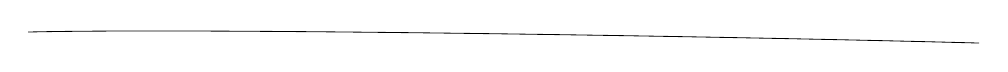
\begin{tikzpicture}[x=\linewidth,y=1cm]
\draw[line width=.3pt] (0,0) .. controls (.18,.05) and (.72,-.05) .. (.996,-.14);
\end{tikzpicture}}

(F) \uline{Portée et limites de la topologie} fppf

Depuis les essais de Serre de trouver une ``coh. de Weil'' en utilisant la cohomologie d'un schéma à coefficients non seulement discrets $\mathbb Z/p^n\mathbb Z$ ($n\mathrel{\mapstochar\relbar\joinrel\dashv}\infty$), ou $\mu_{p^n}$ ($n\mathrel{\mapstochar\relbar\joinrel\dashv}\infty$), mais aussi continus (\inserted{p.ex} $W_n$, $n\mathrel{\relbar\joinrel\dashv}\infty$), qui donnait de bons résultats pour récupérer un $H^1$ correct, pendant de nombreuses années j'étais \inserted{resté} sur l'impression, que j'essayais en vain de préciser, qu'une ``coh. de Weil'' ``$p$-adique'': correcte, en car. $p>0$, \unsure{devait|devrait} pouvoir sortir d'une façon \unsure{ou|--} d'une autre de la cohomologie fppf, pour des coefficients finis p.ex., ou des coefficients
% archive sheet number: 166

\scanpage{167}
\mspage{22}
plus généraux, groupes algébriques sur $k$. La construction en (B) de complexes de \unsure{jacobiennes|jacobiens|jacobienne} locales était, évidemment, \inserted{un peu} lié à cet espoir -- l'homologie donnerait peut-être ce que la cohomologie nous cèle ! Depuis lors, on dispose du formalisme de la cohomologie cristalline, et on sait \inserted{(Berthelot)} que (du moins \deleted{que} pour $X$ projectif et lisse) elle a les propriétés correctes. Si on l'utilise comme une sorte d'étalon sûr à quoi ``mesurer'' les autres cohomologies, on trouve ceci : la partie de la cohomologie cristalline $H^i_{\unsure{\mathrm{cris}|\mathrm{crs}}}(X)$ qui peut être décrite en termes de cohomologie fppf de $X$ à coefficients dans des $k$-groupes algébriques, n'est qu'une \deleted{faible} petite partie du $H^i$ ; de façon précise, utilisant la structure \inserted{très rigide} supplémentaire \unsure{de|des} $H^i$ (\unsure{module|modules} de t.f. sur \unsure{les' anneau|l'anneau} $W(k)$ des vecteurs de Witt) provenant de l'existence de l'hom de Frobenius $H^i\mathrel{\mathop{\unsure{\relbar\joinrel{\scriptscriptstyle\wedge}|\longrightarrow}}\limits^{F}}H^i$ (semi-linéaire) on trouve : que l'on reste toujours dans la partie ``de pente $\leq 1$'' (alors que les pentes possibles varient entre $0$ et $i$\ldots) Ce explique pourquoi pour $i=1$\unsure{.}
% archive sheet number: 167

\scanpage{168}
\mspage{23}
on a pu obtenir via fppf un $H^1$ correct, alors que pour le $H^2$ déjà tous les essais \unsure{ont|nt} été infructueux.

À vrai dire, on conjecture que \uline{toute} la partie de pente $\leq 1$ du $H^i_{\mathrm{cris}}$ provient de fppf : Mais j'ai perdu complètement contact avec ces questions -- des gens comme Mazur, Katz, Messing -- et bien sûr, Deligne -- devraient être au courant du point où en est la question.\unsure{.}

\figure{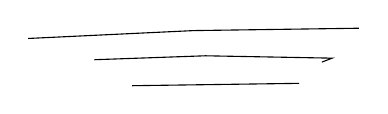
\begin{tikzpicture}[x=1cm,y=1cm]
\draw (0,0) -- (2.1,.10) -- (4.2,.13);
\draw (.84,-.27) -- (2.25,-.22) -- (3.86,-.25) -- (3.73,-.30);
\draw (1.32,-.60) -- (3.44,-.57);
\end{tikzpicture}}

Ta question $7^{\circ}$ semble indiquer qu'il y a malentendu en ton esprit sur la signification du ``type d'homotopie'' de $X$, $X$ un topos (p.ex. le topos \unsure{étale|étal} d'un schéma). Sans doute tu dois confondre l'\unsure{algèbre|algebre} homotopique qu'on peut faire sur $X$ à coups de faisceaux semi-simpliciaux, de champs en \unsure{tous|tout} \unsure{genre|genres}, et des relations entre ceux-ci -- et cet autre point de vue où $X$ (avec sa structure si riche de topos) \unsure{disparait|disparaît} virtuellement,
% archive sheet number: 168

\scanpage{169}
\mspage{24}
pour ne devenir plus qu'un pâle élément d'une ``\unsure{catégorie|categorie} homotopique'' (ou pro-homotopique), déduite de celle des topos par un processus de localisation à brin de zinc -- à première vue, tout ce qui reste encore à ce pauvre $X$, ce sont ses $\pi_i$ -- et ses groupes de \unsure{cohomologies|cohomologie} à \unsure{coéfficient|coefficient} constants -- ou à la rigueur constant tordus. Quand on fouille un peu plus dans cette direction ``que reste-t-il encore à ce pauvre $X$'' on tombe précisément sur les \inserted{$n$-}champs \uline{loc}. \uline{constants} (car un $X\mathrel{\unsure{\relbar\mkern-8mu f|\overset{f}{\longrightarrow}}}X'$ qui est une équivalence d'homotopie induit une $(n+1)$-équivalence entre les cat. de $n$-champs loc. constant sur $X$ et sur $X'$) -- qui contiennent bien sûr les complexes \inserted{de chaines} \unsure{abéliens|abélien} \inserted{de long. $n$} à faisceaux de coh. loc. constants, et l'hypercohomologie de ceux-ci. C'est ainsi qu'on arrive à \deleted{\unsure{la notion|la notion du}} \inserted{\unsure{ce|ca}} triangle de \inserted{\unsure{\textquoteleft|``}\uline{Objets}\unsure{\textquoteright|''|{}}} se déterminant mutuellement
\diagram{\begin{tikzcd}[ampersand replacement=\&,column sep=-1.25em,row sep=large]
\& \begin{gathered}
\text{topos (ou \unsure{espace|espaces} top., ou}\\
\text{ens. }{}^{1}\!/\!{}_{2}\,\text{simpl) }\text{\uuline{\unsure{modulo|modúlo}}}\\
n\text{-}\text{\uline{homotopie}}
\end{gathered} \arrow[dl,leftrightarrow] \arrow[dr,leftrightarrow] \& \\
\begin{gathered}
n\text{-}\text{\unsure{groupoïdes|groupoides}}\\
\text{(à }n\text{-équiv. \unsure{pr.|p.|près})}
\end{gathered} \arrow[rr,leftrightarrow] \& \& \begin{gathered}
n\text{-catégories ``spéciales'' (à}\\
n\text{\unsure{..|-}équivalence près)}
\end{gathered}
\end{tikzcd}}
% archive sheet number: 169

